\documentclass{article}
\usepackage[UTF8]{ctex}
\usepackage[left=2cm,right=2cm,top=1.5cm,bottom=1.5cm]{geometry}
\usepackage{listings}
\usepackage{xcolor}
\usepackage{fontspec}
\usepackage{amsmath}
\usepackage{tikz}
\usepackage[thmmarks,amsmath]{ntheorem}
\setmonofont{Consolas}
\lstset{numbers=left, numberstyle=\tiny, keywordstyle=\color{blue!70}, commentstyle=\color{red!50!green!50!blue!50}, rulesepcolor=\color{red!20!green!20!blue!20}, frame=shadowbox, basicstyle=\ttfamily, breaklines=true, tabsize=4}

\begin{document}
	\title{HW 6}
	\author{肖桐 PB18000037}
	\date{2020 年 11 月 24 日}
	\maketitle

	\newtheorem*{solution}{解}

	\begin{solution}\textnormal{\textbf{1.}}
		加入了切割成本之后, 与原来的$Bottom-Up$解决方案在于, 选择不切割时的收益不需要减去切割成本.
		因此只需要将不切割时的收益设置为初值, 则不需要在求解子问题时单独讨论不切割的情形, 其他的和原来代码一致即可.
		{\rm
		\begin{lstlisting}[language=C]
BUTTOM_UP_CUT_ROD(p, n)
{
	let r[0...n] be a new array
	r[0] = 0;
	for i = 1 to n:
		r[i] = p[i];
		for j = 1 to i - 1:
			r[i] = max(r[i], r[j] + r[i - j] - c);
	return r[n];
}
		\end{lstlisting}
		}
	\end{solution}
	\begin{solution}\textnormal{\textbf{2.}}
		在有向无环图中, 求两个顶点之间的最长路径问题具有最优子结构.\newline
		因此采取自顶向下的方法, 记$l[s, t]$为顶点$s$到顶点$t$之间的最长路径的长度.\newline
		记顶点集合:$U = \{u | ut \in E\}$, 则有:$l[s, t] = \max\limits_{u \in U}\{l[s, u] + 1\}$.\newline
	\end{solution}
	\begin{solution}\textnormal{\textbf{3.}}
		根据课本的算法, 通过计算表$e$、$root$, 可以得到最优二叉搜索树的结构如下:
		\newline
		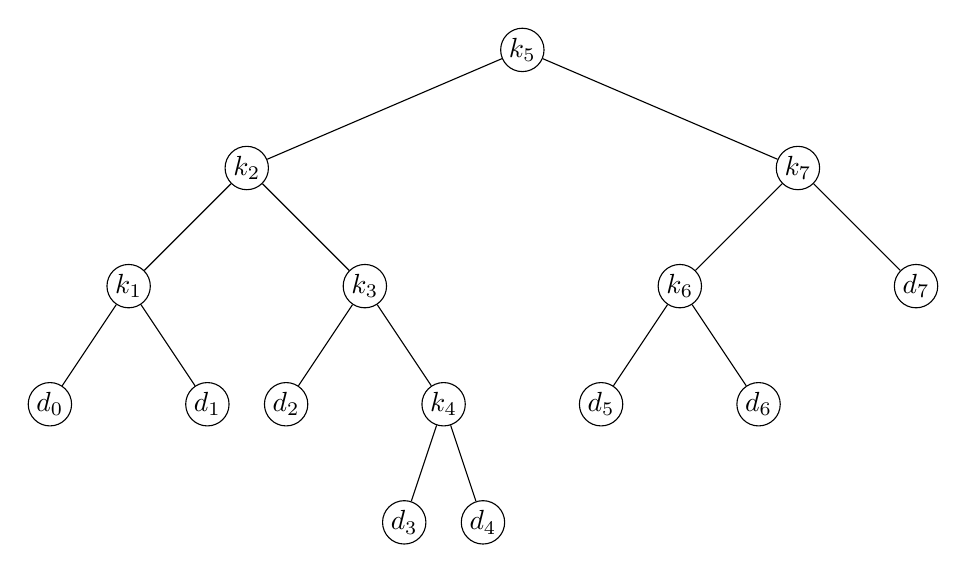
\begin{tikzpicture}[level distance=15mm,
							every node/.style={circle,draw,inner sep=1pt},
							level 1/.style={sibling distance=70mm},
							level 2/.style={sibling distance=30mm},
							level 3/.style={sibling distance=20mm},
							level 4/.style={sibling distance=10mm},]
			\node[circle, draw]{$k_5$}
				child
				{	
					node{$k_2$}
						child
						{
							node{$k_1$}
							child{node{$d_0$}}
							child{node{$d_1$}}
						}
						child
						{
							node{$k_3$}
							child{node{$d_2$}}
							child
							{
								node{$k_4$}
								child{node{$d_3$}}
								child{node{$d_4$}}
							}
						}
				}
				child
				{
					node{$k_7$}
					child
					{
						node{$k_6$}
						child{node{$d_5$}}
						child{node{$d_6$}}
					}
					child{node{$d_7$}}
				};
		\end{tikzpicture}
		\newline
		且该最优二叉搜索树的期望代价为$\sum\limits_{i = 1}^{n}(depth(k_i) + 1)\cdot p_i + \sum\limits_{i = 0}^{n}(depth(d_i) + 1)\cdot q_i = 3.12$.
	\end{solution}
	\begin{solution}\textnormal{\textbf{4.}}
		该问题具有最优子结构. 若结构树中$Root$代表的人参加宴会, 则问题最优解$($即以$Root$为根的最优解$)$为$Root$的宴会交际能力$Root.act$加上以$Root.left.left$为根的子树的最优解.
		若$Root$不参加宴会, 则问题最优解为以$Root.left$为根的子树的最优解. 该性质由$cut-paste$方法易证.\newline
		假设员工的编号为$i$, 为了记号的方便, 该员工在结构树中的节点也用$i$进行标记. 因此可以设计算法:\newline
		初始化一个数组$A[n]$, $n$为公司职工的总人数. 初始设置, 对所有叶子节点对应的员工对应的编号$i$, 令$A[i]$为该员工的宴会交际能力值.\newline
		则有:$A[i] = \max\{A[i.left], A[i.left.left] + i.act + A[i.right]\}$.\newline
		原因是对于以$i$为根节点的子树, 若$i$参加, 则除了需要加上$i.left.left$的最优解之外, 还要加上与$i$同级的员工为根的子树的最优宴会交际能力, 最后加上$i$本身的宴会交际能力.
		将得到的结果与以$i.left$为根的子树的最优宴会交际能力进行比较, 取最大值就是以$i$为根的子树的最优宴会交际能力.
	\end{solution}
	\begin{solution}\textnormal{\textbf{5.}}
		设计算法:\newline
		1. 令一个单位区间的左端点等于当前点集合中, 最左侧的点$x_i$.\newline
		2. 假设该区间包含了点集合中的点$x_i, \cdots, x_j$, 则从点集合中去掉$x_i, \cdots, x_j$.\newline
		3. 若点集合为空, 算法结束; 否则执行第$1$步.\newline
		每一步选取单位区间的左端点都是当前点集中最左侧的点, 假设当前点集中最左侧的点为$x_i$, 此时若将区间左端点取到最左侧的点的左侧,
		即对于$0 < k < 1$, 取区间:$[x_i - k, x_i - k + 1]$, 显然在子区间$[x_i - k, x_i]$不可能会存在任何点, 因此这部分区间就相当于被“浪费”了.
		因此将区间左端点取到当前点集中的最左侧的点是最优的. 因此最终的结果也是最优的, 能使得集合个数最少.
	\end{solution}
	\begin{solution}\textnormal{\textbf{6.}}
		1. 记待找零的数额为$T$, 将可供找零的硬币面额从大到小排列, 存放在数组$r[n]$中. $n$为硬币面额种数.
		同时初始化数组$num[n]$, 用于记录找零时每种硬币的使用个数.\newline
		2. 初始化$i = 0$, 初始化当前已找零金额为$M = 0$.\newline
		3. 若$M + r[i] < T$, 则令$M\ +=\ r[i], num[i]\ +=\ 1$, 继续执行$3$;
		若$M + r[i]\ ==\ T$, 则$num[i]\ +=\ 1$, 算法结束;
		若$M + r[i] > T$, 则$i++$, 继续执行$3$.
		假设在算法执行过程中, 有一次找零本可以使用面额较大的硬币$($面额设为$S$$)$, 却选择了用面额更小的硬币进行找零.
		则为了将这$S$元用面额更小的硬币进行补全, 则必定会使用超过$1$个硬币. 从而使用的总的硬币个数相较于原来的算法更多. 因此该算法是最优的.
	\end{solution}
\end{document}